% Created 2024-10-27 Sun 19:34
% Intended LaTeX compiler: pdflatex
\documentclass[11pt]{article}
\usepackage[utf8]{inputenc}
\usepackage[T1]{fontenc}
\usepackage{graphicx}
\usepackage{longtable}
\usepackage{wrapfig}
\usepackage{rotating}
\usepackage[normalem]{ulem}
\usepackage{amsmath}
\usepackage{amssymb}
\usepackage{capt-of}
\usepackage{hyperref}
\usepackage[margin=0.5in]{geometry}
\hypersetup{colorlinks, linkcolor=black}
\usepackage{geometry}
\geometry{top=2cm}
\geometry{bottom=2cm}
\usepackage{fancyhdr}
\pagestyle{fancy}
\fancyhf[L]{Sistemas Operativos en Red}
\fancyhf[R]{Tema 01}
\fancyfoot[R]{ismael.macareno@educa.madrid.org}
\fancyfoot[L]{CC BY-NC-SA 4.0}
\usepackage{parskip}
\usepackage{mdframed}
\usepackage{fancyvrb}
\usepackage{xcolor}
\definecolor{shadecolor}{RGB}{220,220,220}
\newenvironment{shadedcode}{%
\VerbatimEnvironment
\begin{mdframed}[backgroundcolor=shadecolor,linewidth=0pt]}%
{\end{mdframed}}
\usepackage{attachfile2}
\newcommand{\textattachfilecolor}[2]{\textattachfile[color=0 0 0.5]{#1}{\textcolor{blue}{#2}}}
\usepackage[spanish]{babel}
\usepackage{datetime2}
\DTMlangsetup[es-ES]{ord=raise}
\renewcommand{\dateseparator}{/}
\usepackage{titlesec}
\usepackage{afterpage}
\newcommand\blankpage{\null\thispagestyle{empty}\newpage}
\usepackage{colortbl}
\usepackage{pdfpages}
\usepackage{tcolorbox}
\usepackage{listings}
\usepackage[spanish]{babel}
\lstset{
inputencoding=utf8,
extendedchars=true,
literate={ñ}{{\~n}}1 {Ñ}{{\~N}}1 {á}{{\'a}}1 {é}{{\'e}}1 {í}{{\'i}}1 {ó}{{\'o}}1 {ú}{{\'u}}1 {Á}{{\'A}}1 {É}{{\'E}}1 {Í}{{\'I}}1 {Ó}{{\'O}}1 {Ú}{{\'U}}1,
basicstyle=\ttfamily,
breaklines=true,
columns=fullflexible,
keepspaces=true,
language=TeX,
morekeywords={*, -, **, /}
}
\author{Ismael Macareno Chouikh}
\date{\today}
\title{Preparación Primer Exámen SOR}
\hypersetup{
 pdfauthor={Ismael Macareno Chouikh},
 pdftitle={Preparación Primer Exámen SOR},
 pdfkeywords={},
 pdfsubject={},
 pdfcreator={Emacs 29.4 (Org mode 9.6.15)}, 
 pdflang={Spanish}}
\begin{document}

\maketitle
\tableofcontents

\blankpage

\section{Teoría}
\label{sec:orgcbfe698}
\begin{enumerate}
\item Dime las clasificaciones por SO que conoces
\item ¿Cuáles son los distintos tipos de SO por su forma?
\item ¿Cuáles son las ventajas de las máquinas virtuales?
\item ¿Cuál es la diferencia entre VDI y OVA?
\item Explica las siguientes configuraciones de red de VirtualBox:
\begin{itemize}
\item \textbf{NAT}
\item \textbf{Bridged}
\item \textbf{Red Interna}
\end{itemize}
\item Dime todas las diferencias que conozcas entre las versiones \emph{Home} y \emph{Pro} de \emph{Microsoft Windows}
\item Explícame MBR
\item Explícamen GPT
\item Dime todo lo que sepas sobre los siguientes \emph{filesystems}:
\begin{itemize}
\item FAT16
\item FAT32
\item exFat
\item NTFS
\end{itemize}
\item Define y clasifica:
\begin{itemize}
\item Licencia OEM
\item Licencia por volumen
\item \emph{Software freeware}
\item \emph{Software shareware}
\item Licencia GNU
\end{itemize}
\end{enumerate}

\section{Práctica}
\label{sec:org9c652bd}
\textbf{A NO SER QUE SE INDIQUE, NO SE PUEDE REALIZAR NADA DE MANERA GRÁFICA}
\subsection{CMD}
\label{sec:org465626f}
\begin{enumerate}
\item ¿Qué versión de \emph{Windows} tenemos instalado? Usa los 2 comandos conocidos
\item Crea \textbf{sin gráfico} la partición de DATOS. Puedes añadir otro disco o particionar el que tengas
\item Defragmenta la partición que acabas de crear
\item Crea la siguiente estructura de directorios
\begin{center}
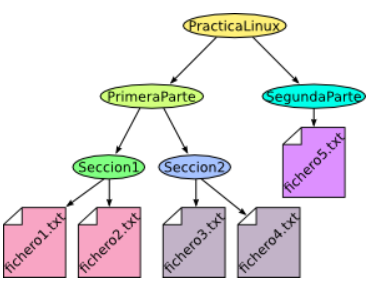
\includegraphics[width=.9\linewidth]{../tipo-examen/img/1.png}
\end{center}
\item Crea un directorio en \texttt{C:\textbackslash{}} que se llame PRACTICA1 y copia el fichero \texttt{LABEL.EXE} del subdirectorio \texttt{SYSTEM32} de Windows en
PRIMERAPARTE pero con el nombre \texttt{ETIQUETA.EXE}. \textbf{Usa dos comandos}
\item Crea un fichero llamado manual.txt
\item Modifica los atributos del fichero creado anteriormente para que tenga los atributos de \textbf{sistema} y \textbf{oculto}.
\item Sin moverte de la carpeta de usuario, y utilizando ruta relativa, copia todos los archivos (sin copiar subcarpetas) de la carpeta
windows de C en la carpeta PRUEBA
\item Haz una copia idéntica de la carpeta prueba a la carpeta copiaPrueba, en la misma partición
\item Borrar la carpeta copiaPrueba, y mirando la ayuda del comando xcopy, vuelve a copiar la carpeta, de forma que se copien todos
los archivos.
\item En la carpeta prueba. Pon atributos de sistema y oculto a los archivos que empiezan por w y tienen la extensión .log
\item Quita todos los atributos en los archivos de la carpeta prueba
\end{enumerate}

\subsection{Powershell}
\label{sec:org6acdd92}
\subsubsection{Estructura de Directorios}
\label{sec:org545fcf6}
\begin{enumerate}
\item Ejecuta Powershell sin privilegios de administración
\item Crea un directorio "tunombreyapellido"
\item Sitúate en el
\item Crea la siguiente estructura
\begin{center}
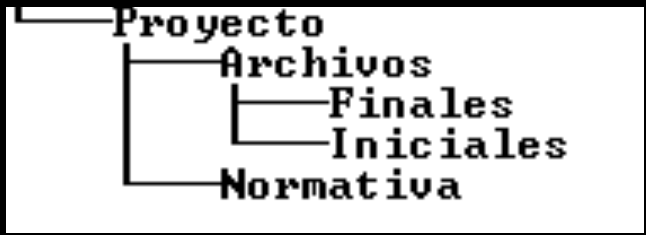
\includegraphics[width=.9\linewidth]{../tipo-examen/img/2.png}
\end{center}
\item Cambia el nombre de finales por fin
\item Copia el directorio archivos en normativa
\item Mueve el directorio fin a proyecto
\item Consulta la ayuda del \texttt{copy-item}. Consulta los ejemplos de ayuda
\item Ejecuta el siguiente comando y explica lo que hace:
\begin{itemize}
\item \texttt{Copy-item proyecto .. -recurse}
\end{itemize}
\item Vuelve a dejar la estructura de directorios como estaba en el ejercicio 4
\end{enumerate}
\subsubsection{Trabajando con archivos}
\label{sec:orgde5d9d8}
\begin{enumerate}
\item Desde el Powershell crea los archivos Norm1.txt y Norm2.txt en el directorio normativa, y p1.bat y p2.bat
en proyecto. De momento estarán vacíos
\item Comprueba el contenido de los ficheros anteriores
\item Copia los archivos Norm1 y Norm2 al directorio archivos. Modifica su nombre a Norm1\textsubscript{antiguo} y Norm2\textsubscript{antiguo} en directorio
archivos
\end{enumerate}
\subsection{Programar tareas GUI}
\label{sec:org430ab01}
\begin{enumerate}
\item Realizar un archivo por lote que obtenga los ficheros modificados hoy. Como este fichero vamos a ejecutarlo otros días, en la línea
que se filtra por fecha, introducimos la fecha como variable de \emph{Windows}. Para ello usammos: \texttt{find "\%date\%"}
\item Añade al anterior fichero, una línea que sirva para apagar el equipo.
\item Programar para que todos los días a las 14:30 se ejecute el fichero creado anteriormente
\end{enumerate}
\subsection{Programar tareas CLI}
\label{sec:org68437ac}
\begin{enumerate}
\item Programas un \emph{script} que deje guardados todos los inicios de sesión:
\begin{itemize}
\item Crear 3 usuarios en \emph{Windows}
\begin{itemize}
\item Nombre
\item Primer apellido
\item Segundo apellido
\end{itemize}
\item Crear un fichero por lotes, que guarde cuando se ejecute en un fichero
\begin{itemize}
\item \textbf{el usuario \ldots{}. ha iniciado sesión el día \ldots{}. a las \ldots{}. horas}
\item Se tendrá en cuenta que en el fichero quedará guardado todas las veces que se ejecute el \emph{script}
\end{itemize}
\item Programar con el comando \texttt{schtasks} para que se ejecute el \emph{script} cada vez que un usuario inicie sesión
\item Comprobar el funcionamiento iniciando sesión al menos una vez con los 3 usuarios
\end{itemize}
\end{enumerate}
\end{document}
